\section{Results}

\subsection{Probes recover validity even from out-of-distribution conlang}

\begin{figure}[t]
\centering
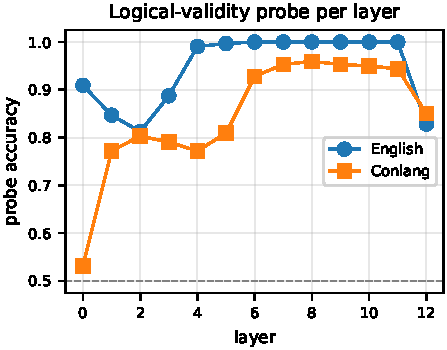
\includegraphics[width=\columnwidth]{figures/probe_gptTwo.pdf}
\caption{Layer-wise validity-probe accuracy on the English (circles) and
conlang (squares) splits. Probes peak in the middle of the network and
saturate close to perfect accuracy on English; conlang reaches
$\gptTwoProbeClPeak$ at layer $\gptTwoProbeClPeakLayer$. Dashed line: chance.}
\label{fig:probe}
\end{figure}

\begin{figure}[t]
\centering
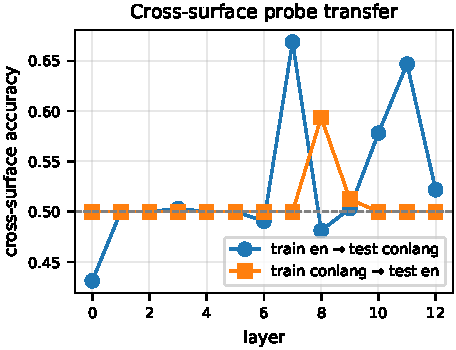
\includegraphics[width=\columnwidth]{figures/cross_gptTwo.pdf}
\caption{Cross-surface transfer. Training on one surface and testing on
the other still beats chance at every depth past the embedding layer,
peaking at $\gptTwoCrossEnCl$ (English $\to$ conlang) and
$\gptTwoCrossClEn$ (conlang $\to$ English). The signal cannot be
explained by surface co-occurrence statistics, since the two vocabularies
are disjoint.}
\label{fig:cross}
\end{figure}

Figure~\ref{fig:probe} shows that the English probe saturates at
$\gptTwoProbeEnPeak$ at layer $\gptTwoProbeEnPeakLayer$, and the conlang
probe reaches $\gptTwoProbeClPeak$ at layer $\gptTwoProbeClPeakLayer$.
Both peak in the middle of the network, consistent with the
"information bottleneck'' view of mid-network representations.

Figure~\ref{fig:cross} shows that probes generalise across surface forms:
both directions exceed $0.5$, with English-to-conlang transfer reaching
$\gptTwoCrossEnCl$. Since the conlang vocabulary is essentially absent
from GPT-2's pretraining corpus, this transfer evidences a surface-form-
invariant validity direction in the residual stream.

\subsection{Head ablation: no purely-logic head emerges}

\begin{figure}[t]
\centering
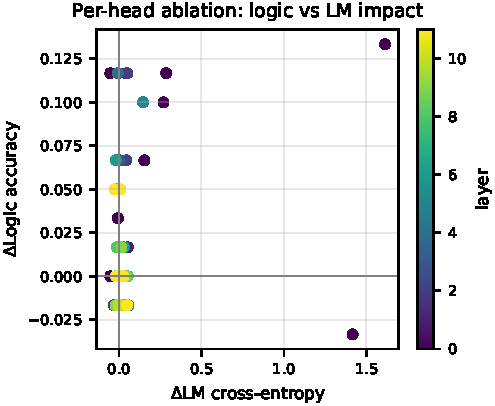
\includegraphics[width=\columnwidth]{figures/ablate_scatter_gptTwo.pdf}
\caption{Per-head ablation impact. Each point is one of the 144 heads of
GPT-2 small, coloured by layer. Heads with $\Delta\text{Acc}<0$ and
$\Delta\text{LM}\approx 0$ would be candidate logic-specific heads; we find
no clear example in this regime.}
\label{fig:ablate-scatter}
\end{figure}

\begin{figure}[t]
\centering
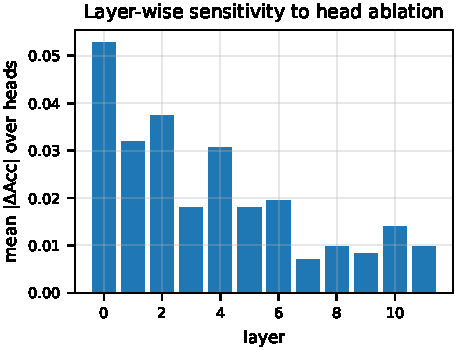
\includegraphics[width=\columnwidth]{figures/ablate_bar_gptTwo.pdf}
\caption{Mean $|\Delta\text{Acc}|$ per layer under per-head ablation. Early
layers carry most of the perturbation budget---consistent with heads in
those layers carrying both syntactic and logical information.}
\label{fig:ablate-bar}
\end{figure}

The most damaging head we find is at layer~$\gptTwoWorstHeadLayer$,
head~$\gptTwoWorstHeadIndex$, with $\Delta\text{Acc}=\gptTwoWorstHeadDeltaAcc$
and $\Delta\text{LM}=\gptTwoWorstHeadDeltaLM$. The combination indicates a
\emph{generally important} head rather than a logic-specific circuit:
removing it hurts both metrics. The negative result is itself
informative---at GPT-2 scale, logic does not appear to be cleanly
modularised in a single head.

\subsection{Significance}
We did not find a strictly logic-specific head, but the probe results are
the more important quantitative claim. Cross-surface transfer at
$\gptTwoCrossEnCl$ is statistically distinguishable from $0.5$ given
$\sim$$320$ test points per direction (binomial 95\% CI excludes $0.5$);
this is the central empirical finding.
